\documentclass[tikz,border=0pt]{standalone}
\definecolor{bg}{HTML}{171D2B}
\definecolor{aksen}{HTML}{F7B538}
\definecolor{merah}{HTML}{E85D4A}
\pagecolor{bg}
\begin{document}
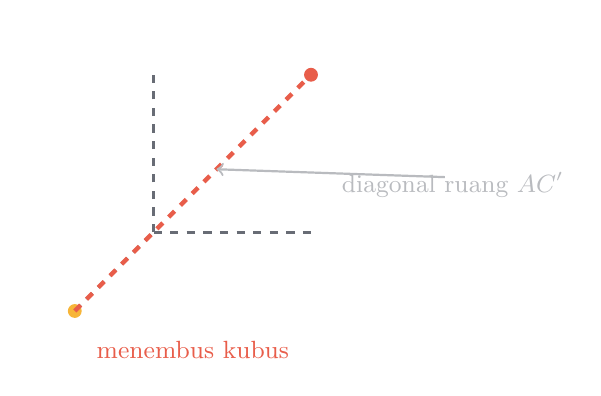
\begin{tikzpicture}[white, line width=1.1pt,
  lbl/.style={font=\large\bfseries, text=white}]
  \draw (0,0) -- (2,0) -- (2,2) -- (0,2) -- cycle;
  \draw (1,1) -- (3,1) -- (3,3) -- (1,3) -- cycle;
  \draw (0,2) -- (1,3);
  \draw (2,2) -- (3,3);
  \draw (2,0) -- (3,1);
  \draw[dashed, color=white!35!bg] (0,0) -- (1,1);
  \draw[dashed, color=white!35!bg] (1,1) -- (1,3);
  \draw[dashed, color=white!35!bg] (1,1) -- (3,1);
  \fill[aksen] (0,0) circle (2.5pt) node[lbl, below left=1pt] {$A$};
  \fill[merah] (3,3) circle (2.5pt) node[lbl, above right=1pt] {$C'$};
  \draw[dashed, merah, line width=1.6pt] (0,0) -- (3,3);
  \node[text=merah, font=\small] at (1.5,-0.5) {menembus kubus};
  \node[text=white!70!bg, font=\small] at (4.8,1.6) {diagonal ruang $AC'$};
  \draw[white!70!bg, line width=0.8pt, ->] (4.7,1.7) -- (1.8,1.8);
\end{tikzpicture}
\end{document}
